\documentclass{article}

\usepackage{a4wide}
\usepackage[utf8]{inputenc}
\usepackage[T1]{fontenc}
\usepackage{natbib}
\usepackage[french]{babel}
\usepackage[babel=true]{csquotes} % guillemets français
\usepackage{graphicx}
\graphicspath{{Images/}}
\usepackage{color}
\usepackage{hyperref}
\hypersetup{colorlinks,linkcolor=,urlcolor=blue}

\usepackage{amsmath}
\usepackage{amssymb}


\title{Rapport du projet de sécurité informatique : CryptoBank}
\author{Nativel Emmanuel,  M1 informatique}
\date{\today}

\begin{document}

\maketitle % pour écrire le titre


%% Le résumé:
\begin{abstract}
  Présentation de CryptoBank,  une application web développée en Javascript, et plus précisément en React JS, dans le cadre de l'UE Sécurité Informatique en M1 informatique. Le code source se trouve sur un dépôt git\cite{GitHub} et une démonstration est disponible en ligne\cite{site} (à consulter avec une version récente de Google Chrome).
\end{abstract}

\section{Introduction}
\label{section:introduction}

Dans le cadre de l'UE Sécurité Informatique en M1 informatique, nous devons proposer une implémentation des algorithmes de cryptographie suivants : \textit{Atbash, César, Vigenère, homophone avec carré de Polybe, Playfair, Hill} (cas où m = 2 uniquement), \textit{transposition rectangulaire et DES} pour la catégorie des algorithmes symétriques et \textit{RSA} pour la catégorie des algorithmes asymétriques. 
Pour se faire, j'ai choisi de développer une application web statique en utilisant le framework Javascript React JS\cite{react}. De plus, certaines de ces implémentations doivent être appliquées à toute la table ASCII étendue.
Afin de vous présenter au mieux l'application CryptoBank, nous allons dans un premier temps faire une présentation de l'environnement de travail et des procédures d'installation. Puis, nous nous intéresserons aux fonctionnalités ajoutées en dehors de l'implémentation des algorithmes de cryptographie. Ensuite, nous nous concentrerons sur certains algorithmes en particulier. Et enfin, nous exposerons les difficultés rencontrées lors du développement de cette application.

\section{Environnement de travail et installation}
\subsection{Quelques mots sur React JS}

React JS est une librairie Javascript développée par Facebook en 2013. Son but est de faciliter la création d'interfaces utilisateurs à travers une approche orientée composants permettant d'isoler chaque portions de l'interface et sa logique indépendemment des autres. Ainsi, chaque composant possède sont état local et retourne une page HTML ou une portion d'une page HTML. React est très populaire aujourd'hui et est utilisé par de nombreuses entreprises dont Netflix, AirBnb, Facebook et d'autres encore. En effet, il offre de nombreux avantages et notamment une grande performance. 

J'ai choisi d'utiliser ce framework en vue de rester proche de mes objectifs professionnels. En effet, cela fait quelques moi maintenant que je me forme parallèlement à l'Université afin d'acquérir des compétences techniques dans le développement web. C'était donc pour moi l'occasion de mettre en application mes acquis.

\cleardoublepage

\subsection{Problèmes de compatibilité}
A l'annonce de l'ajout d'un algorithme asymétrique au projet, une difficulté supplémentaire s'est ajoutée au développement. En effet, l'utilisation de \foreignquote{french}{grands entiers} en Javascript est un peu délicate à l'heure actuelle car le type de variable BigInt destiné à l'utilisation des entiers supérieurs à $2^{53}$ est encore en phase de \foreignquote{french}{brouillon}\cite{bigInt}. Le type BigInt n'est donc pas reconnu par tous les navigateurs. Par conséquent, je vous demande de lancer l'application sous une version récente de google chrome, navigateur sur lequel les tests ont été effectués. De plus, sur la version mise en ligne, l'algorithme RSA ne fonctionnera pas et ne pourra être testé qu'en localhost. 

\subsection{Structure du projet}
Dans cette sous-section, nous allons analyser la structure du projet et repérer les fichiers dédiés à l'implémentation des algorithmes de cryptographie.

A la racine du projet, nous pouvons trouver deux dossiers : 
\begin{itemize}
\item Le dossier \textbf{public} contenant toutes les ressources publique du projet, dont la page\textit{ index.html} qui est le départ de notre application. Dans ce fichier se trouve une div ayant pour id \textbf{root}. C'est dans cet div que React va injecter tout le contenu de notre application. C'est donc le point d'entrée.
\item Le dossier \textbf{src} contenant tous les fichiers sources de notre application. Nous allons porter notre attention sur ce dossier dans cette sous-section.
\end{itemize}

Dans le dossier \textbf{src}, nous avons accès à trois dossiers : \textbf{components}, \textbf{data} et \textbf{scripts}. 
Tout d'abord, le dossier components contient, comme son nom l'indique, tous les composants de l'application. Voici une représentation des composants AppBar et Banner dans l'interface graphique :

\bigskip
\bigskip

\begin{center}
  \includegraphics[scale=0.15]{components1.png}
\end{center}

\cleardoublepage

Et ci-dessous, une représentation des composants Footer et CardsCollection :
\bigskip
\begin{center}
  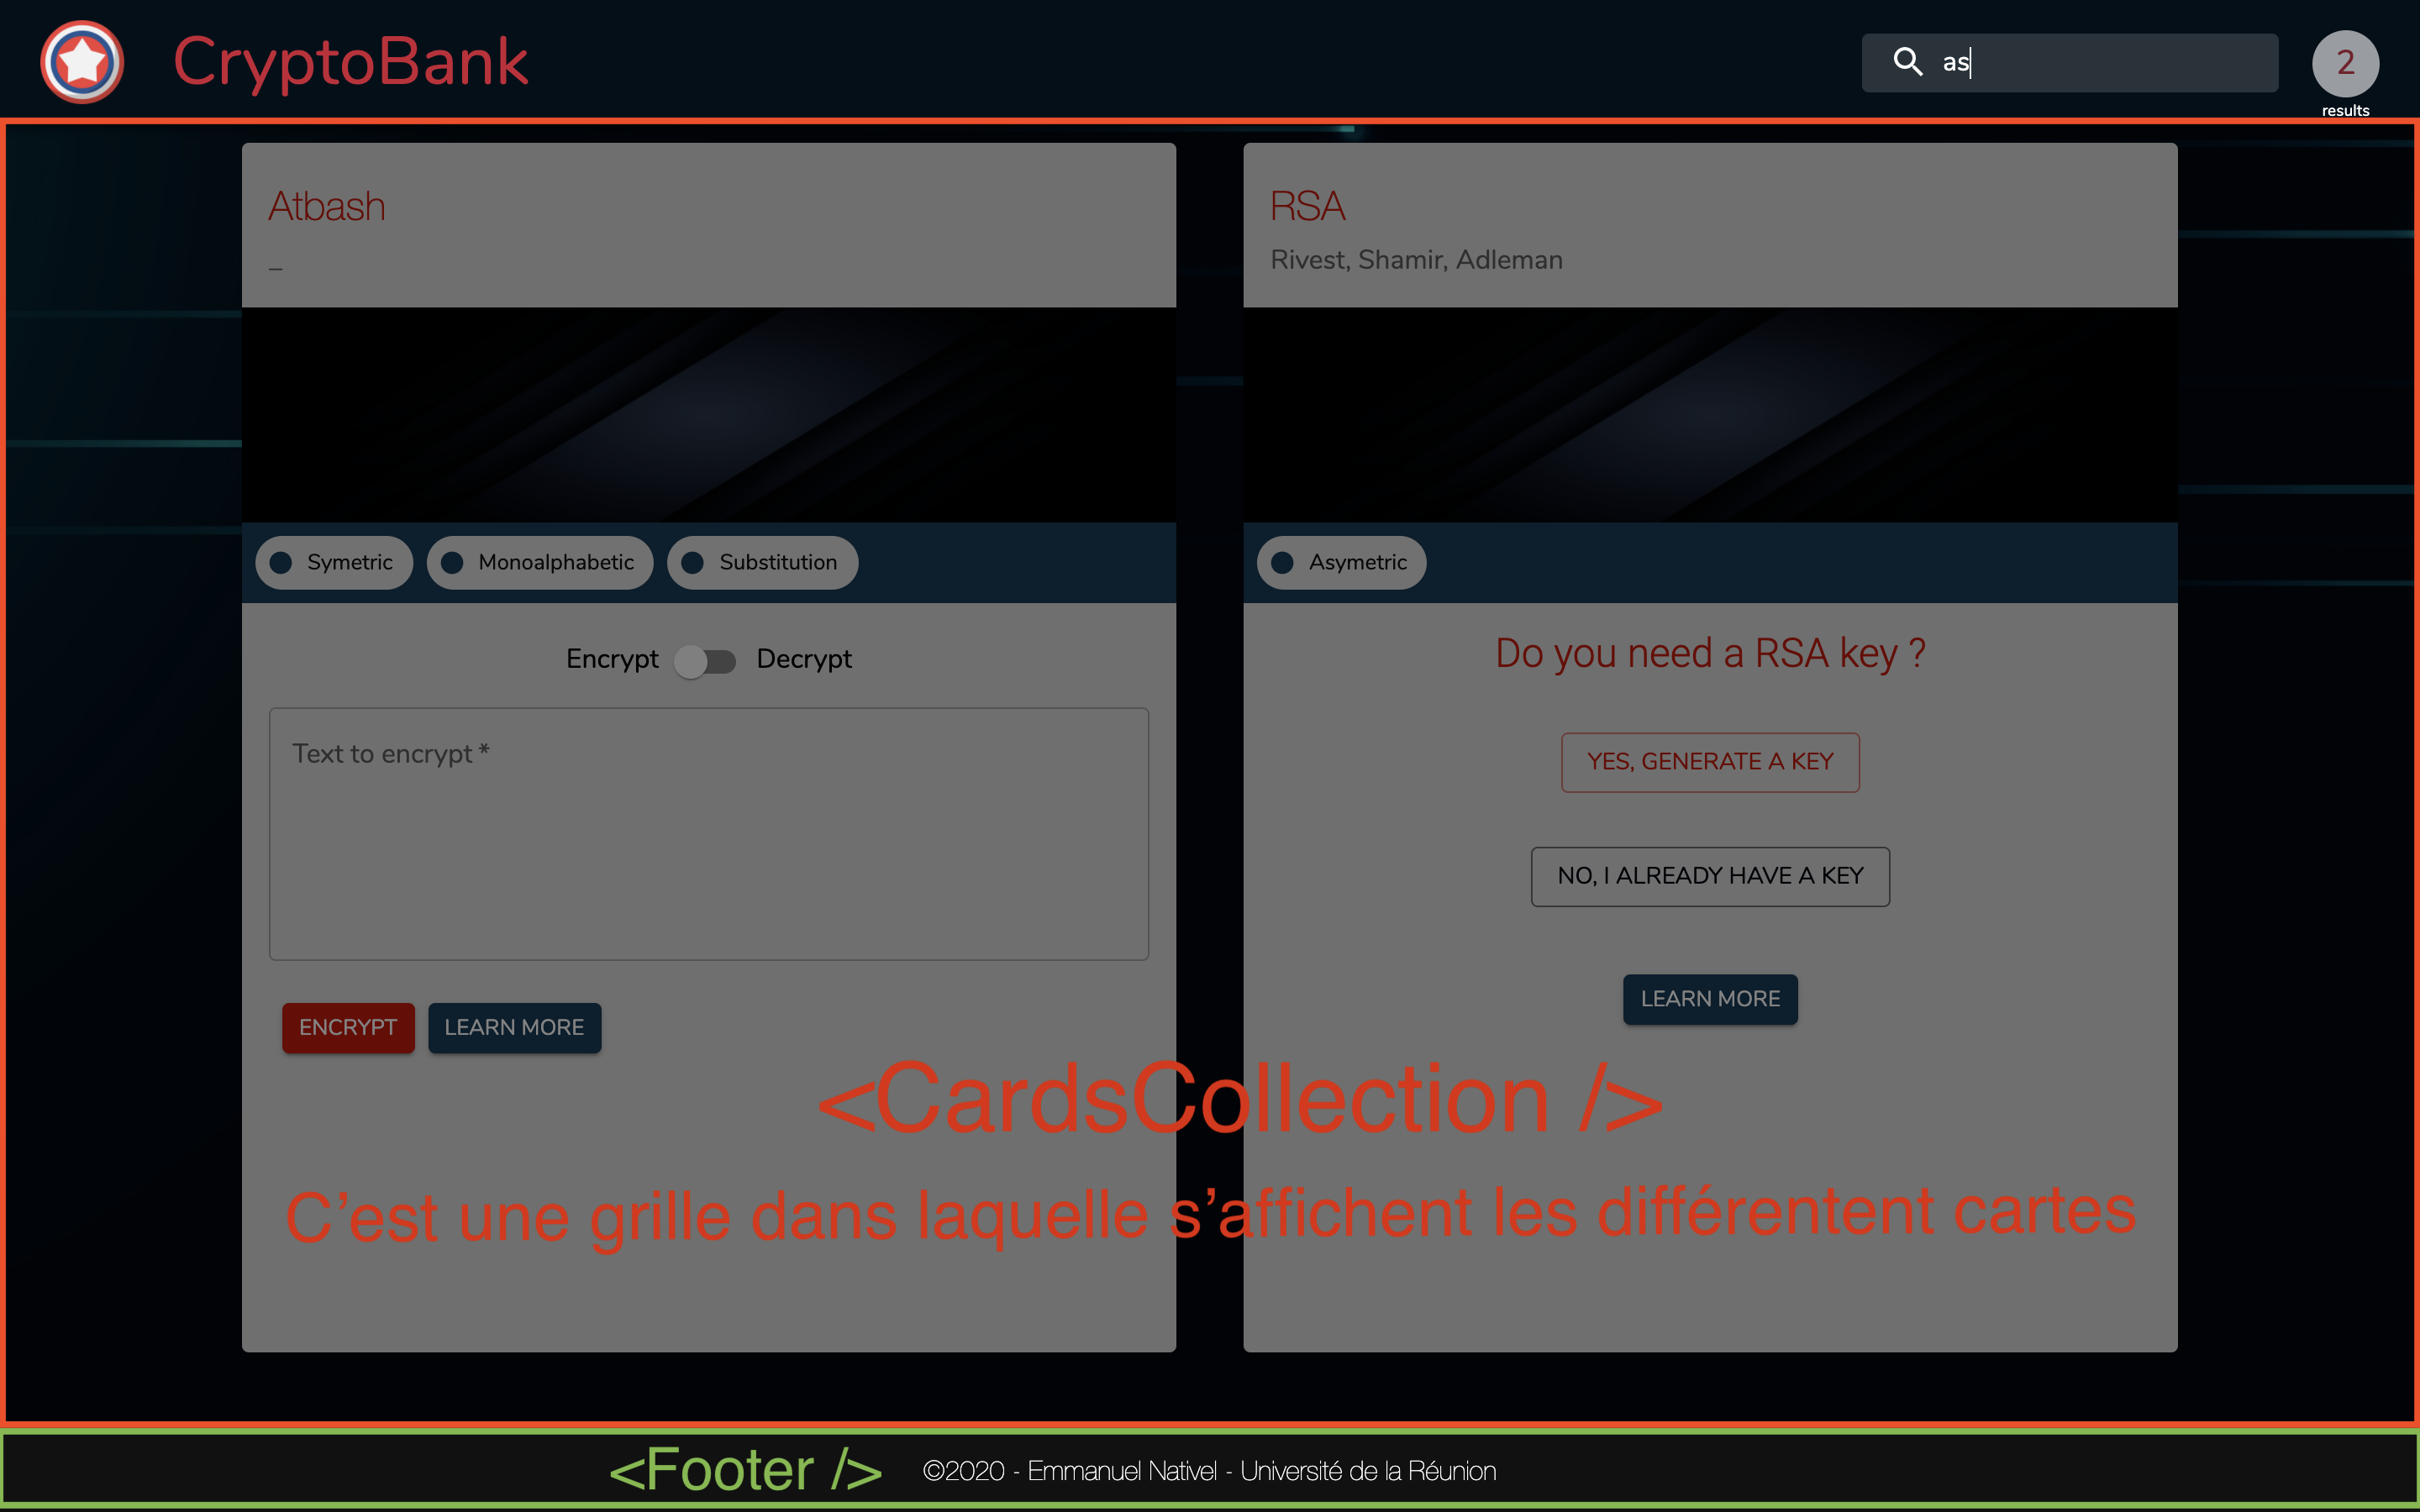
\includegraphics[scale=0.1]{components2.png}
\end{center}
\bigskip

Enfin, comme le montre l'image ci-dessous représentant le composant CardItem, celui-ci est lui même divisé en plusieurs composants. CarItem contient le composant CardResultPanel destiné à afficher le résultat de l'exécution de l'algorithme et un autre composant destiné à afficher le formulaire de la carte. Chaque algorithme de cryptographie implémenté a son propre formulaire situé dans le dossier CardForms. C'est le fichier \textit{AlgoManager.js} qui se charge d'associer le bon formulaire au bon algorithme. 

\bigskip
\begin{center}
  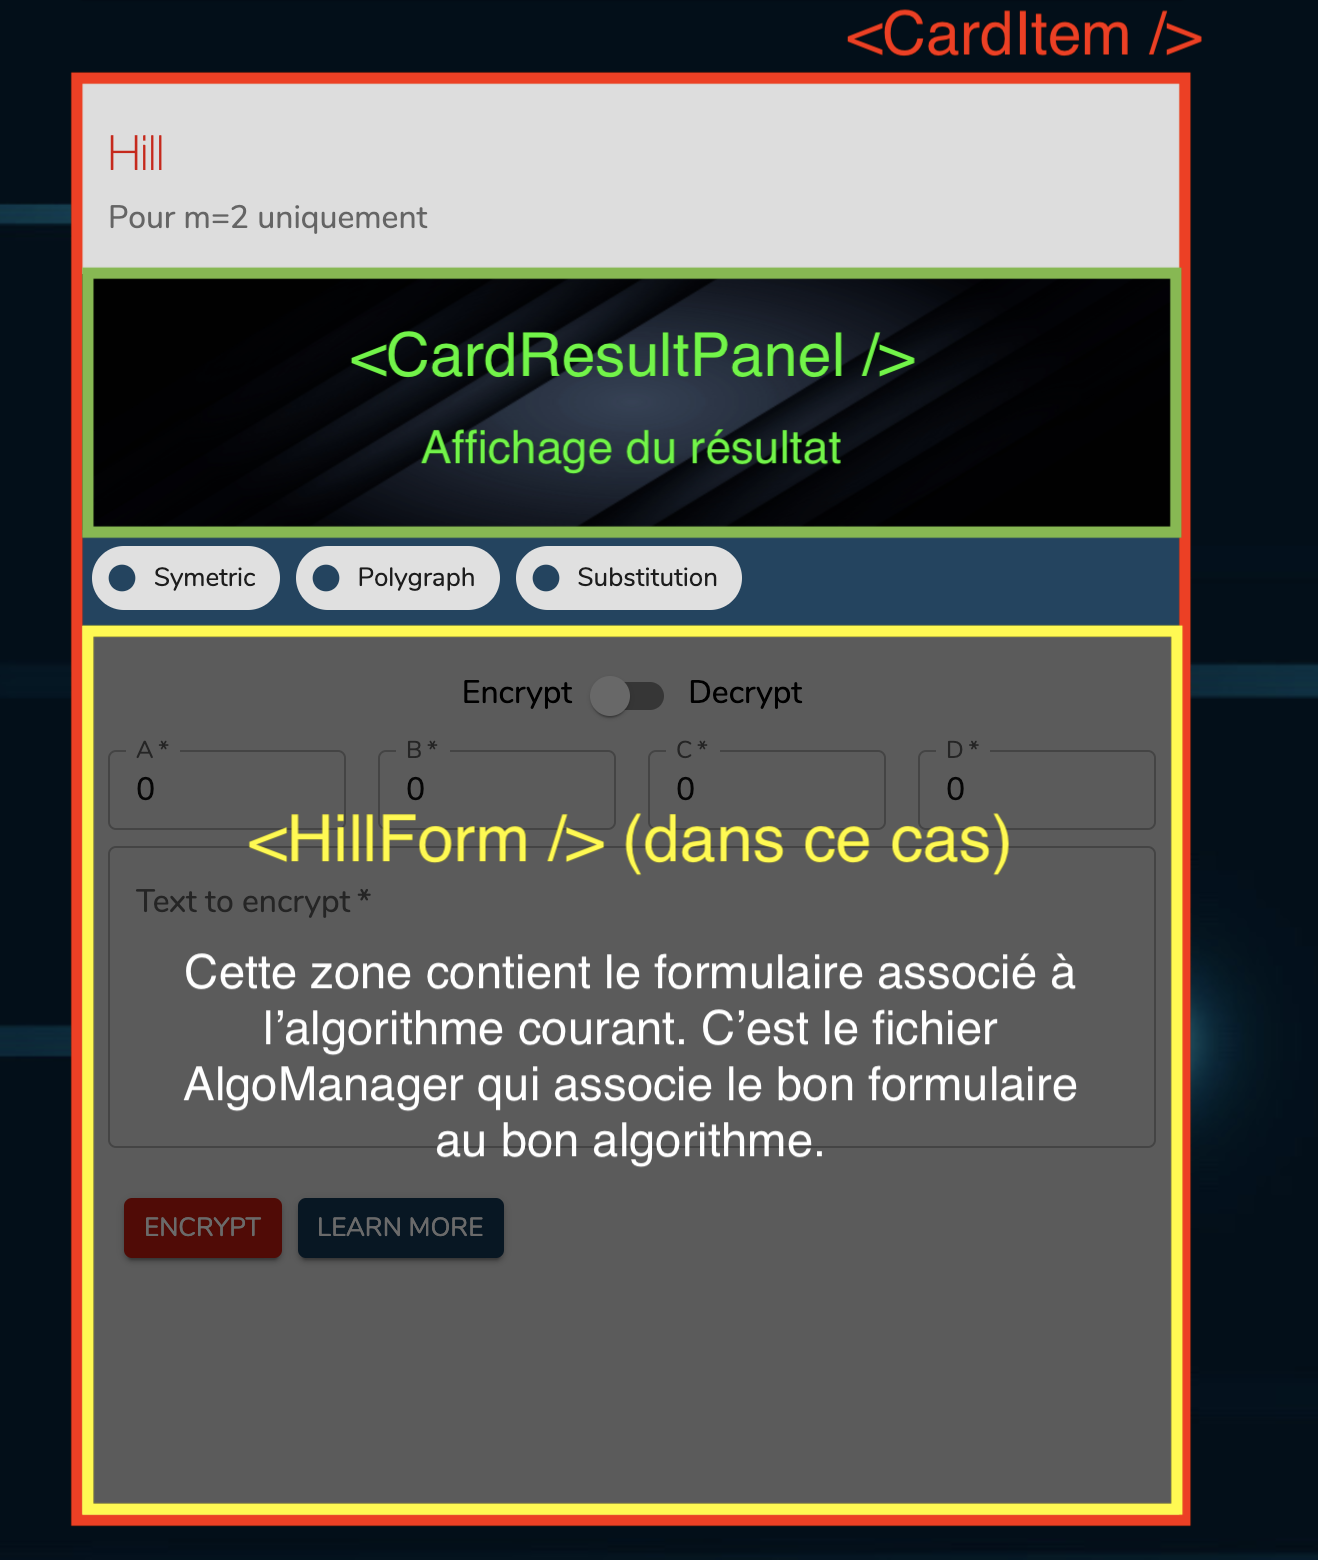
\includegraphics[scale=0.3]{components3.png}
\end{center}
\bigskip

En retournant à la racine du dossier components, nous voyons ensuite le dossier \textbf{data}. Celui-ci contient des méta-données sur chacun des algorithmes de cryptographie. 
Nous avons ensuite le dossier \textbf{scripts}. C'est dans ce dossier que se trouvent les différents algorithmes de cryptographie. Il y a un fichier par algorithme implémenté. De plus parmi ces fichiers nous retrouvons d'autres fichiers utilitaires : \textit{utils.js}, \textit{ASCIIextended.js},\textit{ DESconst.js} et \textit{PrimeNumbers.js}. Ces fichiers contiennent des constantes ou des fonctions utilisées dans les algorithmes.

Afin de comprendre comment les liens sont fait entre ces fichiers, voici un petit exemple de l'importation de fonctions externes dans le fichier DES.js :

\begin{verbatim}
import { BIT_ROTATION, Sboxes, IP, FP, E, P, PC1, PC2 } from "./DESconst";
import { getExtendedAsciiCharOf, splitExtASCIIstring, getExtendedAsciiCodeOf, hexaToDecimal }
from "./utils";
\end{verbatim}

À la ligne 1, nous importons les différentes constantes depuis de fichier DESconst.js. Et à la ligne 2, nous importons des fonctions depuis le fichier utils.js. 


\subsection{Comment lancer l'application ?}
Des instructions détaillant les pré-requis ainsi que la procédure pour lancer l'application sont disponibles dans le fichier \textit{README.md}. Ces instructions se trouvent également sur la page d'accueil du lien github\cite{GitHub}.

\textit{\textbf{NB : }} \textit{Des traces sont parfois affichées dans la console du navigateur lors de l'exécution des algorithmes.}


\section{Les fonctionnalités ajoutées}
\subsection{La recherche}
Dans la barre de recherche, il est possible de rechercher des algorithmes. Cette recherche se fait par mots clés. Les mots contenus dans le titre des algorithmes ainsi que les propriétés de ceux-ci sont reconnus par le moteur de recherche.

Par exemple, les mots suivants, en anglais, peuvent générer des résultats à la recherche : \textit{DES, Hill, asymetric, symetric, Monoalphabetic, Substitution, Polygraph} ou encore\textit{ Super-encryption}... 

Le nombre de résultat(s) s'affiche dans le petit compteur à droite de la barre de recherche. En cliquant sur le compteur ou en appuyant sur la touche entrée, vous serez dirigé vers les résultats qui se trouvent plus bas dans la page.

\subsection{La gestion des erreurs}
Pour chacun des formulaires, une gestion d'erreur est mise en place. Pour le chiffrement de Hill, le déterminant de la matrice est calculé en temps réel et affiche une erreur si celui-ci n'est pas valide. Dans le formulaire du DES, la clé peut être entrée en décimal ou en binaire. Dans les deux cas, les bits de contrôle sont pris en compte de sorte que chaque octets contienne un nombre impair de bits à 1. Les autres algorithmes contiennent également quelques vérifications au niveau de clé du chiffrement. Voici une image montrant un déterminant invalide pour l'algorithme de Hill.

\begin{center}
  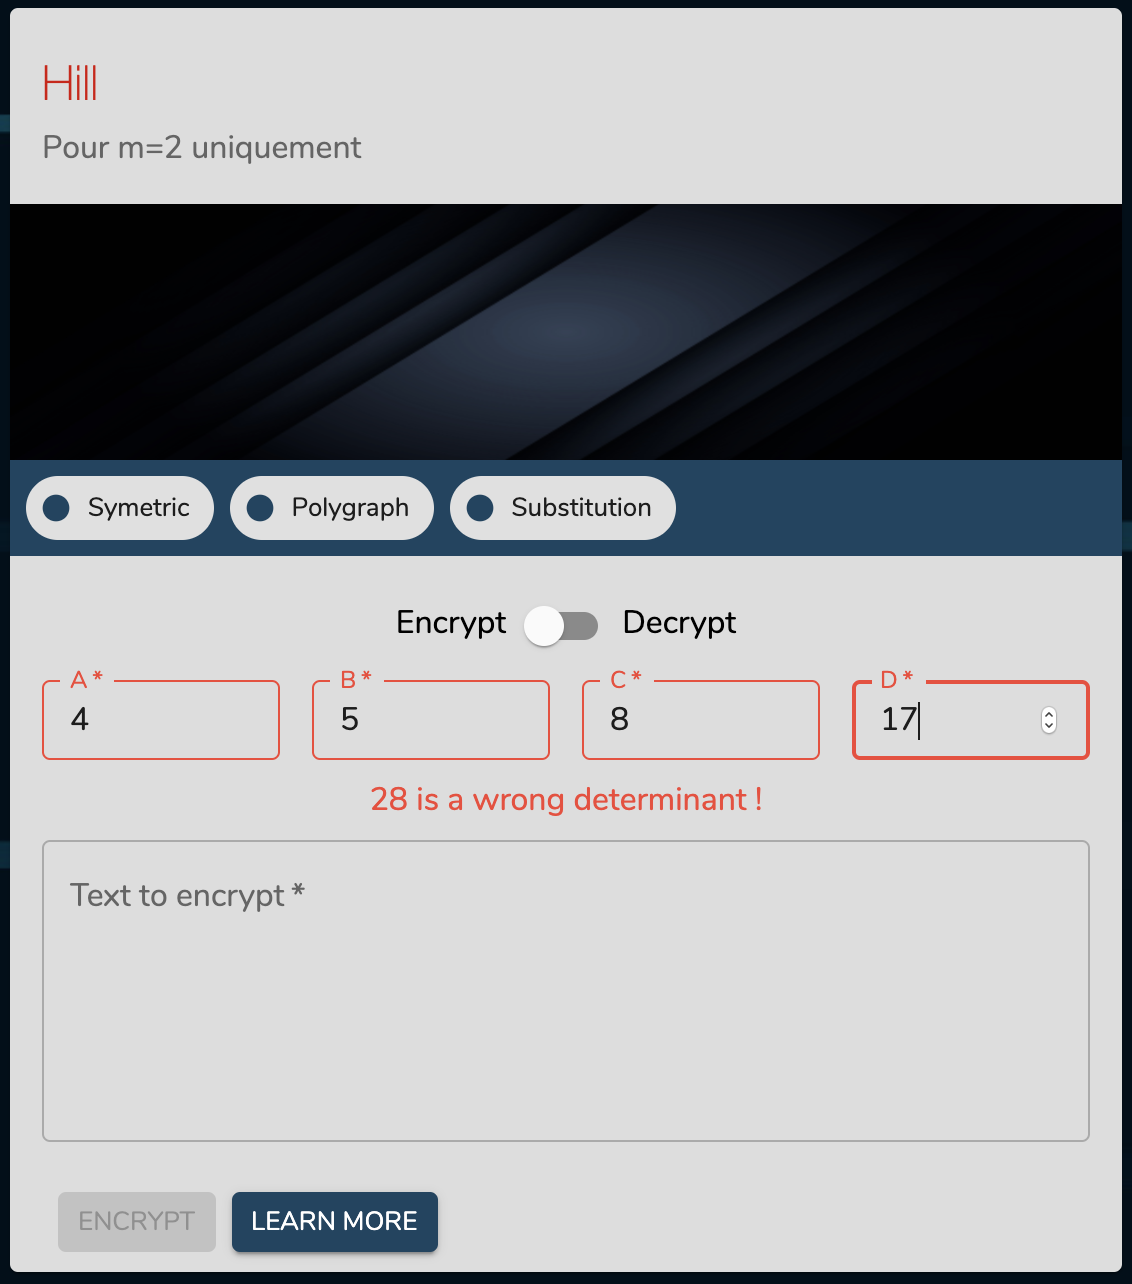
\includegraphics[scale=0.4]{error.png}
\end{center}
\bigskip

\subsection{Une application responsive}
L'application web est également utilisable sur un téléphone. En effet, l'interface utilisateur est prévue pour s'adapter à différentes tailles d'écrans.


\section{Les algorithmes de chiffrement}

Dans cette section, nous allons aborder quelques précisions sur les algorithmes de cryptographie. Le détail des algorithmes n'est pas indiqué ici, il se trouve dans les commentaires du code source.

\subsection{L'ASCII étendu}

Les algorithmes suivants sont appliqués à la table ASCII étendue : \textit{Cesar, Atbash, Vigenère, Hill, transposition rectangulaire et le DES.}
Il est possible d'écrire les caractères sous formes hexadécimale en respectant le format \textbackslash{}xFF.

La partie étendue de la table ASCII est codée en dur dans le fichier \textit{ASCIIextended.js} du dossier scripts.

\subsection{Quelques détails à propos de RSA}
L'interface de la carte pour RSA se compose en trois états : 
\begin{itemize}
\item L'état par \textbf{défaut} dans lequel l'utilisateur choisit de générer une clé s'il n'en a pas ou de crypter/décrypter son message s'il possède déjà une clé RSA. 
\item L'état \textbf{génération de clé} dans lequel l'utilisateur peut renseigner les valeurs de p et de q ou les générer aléatoirement, afin d'obtenir une clé publique et la clé privée associée. 
\item L'état \textbf{principal} dans lequel l'utilisateur va crypter ou décrypter son message.
\end{itemize}

Lorsque l'utilisateur choisit de générer une clé, un warning apparaît si l'algorithme estime que le temps de décryptage sera trop long (en fonction de la valeur de n). Des erreurs sont également générées si p et q ne sont pas premiers ou trop grands.
Une fois que les clés ont été générées, celles-ci sont automatiquement reportées dans le formulaire de cryptage/décryptage.
Les opérations de cryptage et de décryptage du message sont bloquantes. 

Afin d'éviter les attaques par l'analyse de fréquence d'apparition des lettres, les codes ASCII sont découpés en blocs de même longueur. On leur donne d'abord une longueur fixe, ici 3, en rajoutant des 0 devant si nécessaire. Par exemple, la suite de codes ASCII suivante : 72 101 108 112 32 33 est transformée en 072 101 108 112 032 033. Puis, cette suite est regroupée en blocs de 4 et devient donc 0721 0110 8112 0320 0033. Chaque bloc doit être inférieur à n. 
Enfin, pour déchiffrer, il faudra d'abord séparer la suite en blocs de 4 pour obtenir 0721 0110 8112 0320 0033, puis faire des blocs de 3. Nous retrouvons donc le bon code ASCII : 072 101 108 112 032 000 33, soit 72 101 108 112 32 33.
Cette méthode est donnée par le tutoriel d'\textit{openclassroom}\cite{openclassroom}.


\section{Difficultés et impressions}

Je pense que malgré la première impression que donne les algorithmes complexes tels que le DES, Hill ou RSA, ce ne sont pas les plus difficiles à implémenter. En effet, dans mon cas, l'implémentation des algorithmes utilisant un carré de polybe ou des permutations des colonnes d'une matrice, tel que la transposition rectangulaire, était plus délicate. 

Cependant, j'ai pris beaucoup de plaisir à réaliser ce projet, d'autant plus que j'ai eu l'occasion de l'appliquer à ce que j'aime faire : des applications web. 

Plusieurs améliorations sont possibles, comme la gestion des opérations bloquantes, ou la création d'une API côté serveur pour implémenter les algorithmes plutôt que de les implémenter directement côté client. De plus, l'ajout officiel du type BigInt au langage Javascript est prévu prochainement et permettra de faciliter l'implémentation des algorithmes asymétriques.

\bibliographystyle{plain}
\bibliography{ma_biblio}

\end{document}
